% ============================================================
% ============================================================
% NACA0012 -- DROPLET IMPINGEMENT
% ============================================================
% ============================================================

\section[Imp.]{\textbf{Droplet Impingement}}


% ============================================================
% ONERA M6 -- Collection Efficiency Profiles
% ============================================================

\begin{frame}[shrink]{\small ONERA M6 -- Collection Efficiency (15 Bins, L1)}
\scriptsize

% ------------------------------------------------------------
% Middle slice
% ------------------------------------------------------------
\only<1>{
\centering
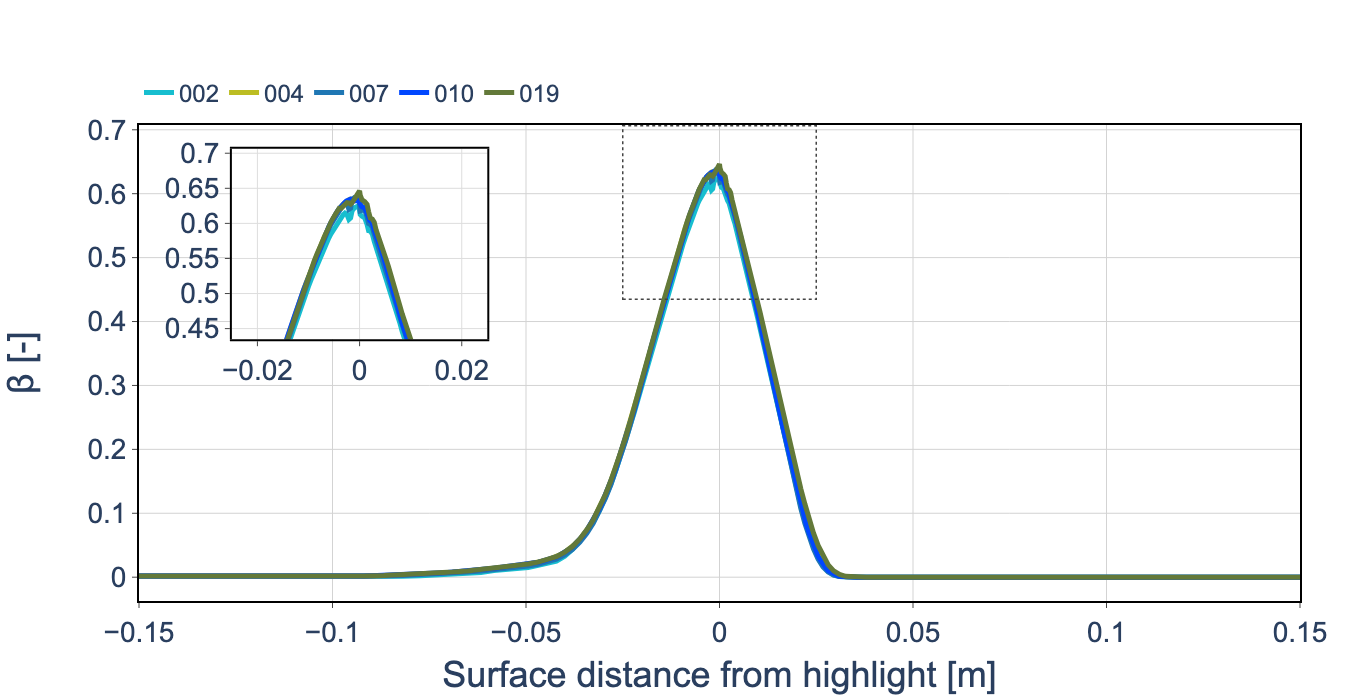
\includegraphics[width=0.62\textwidth]{FIGURES/IMPINGEMENT/tc_oneram6_L1_beta_bins15_vs_s_slice_0p75_roughness_1mm.png}

\vspace{0.05cm}

\textbf{$y=0.75$ m}
}

% ------------------------------------------------------------
% Inboard and outboard slices
% ------------------------------------------------------------
\only<2>{
\begin{columns}[T,onlytextwidth]

\begin{column}{0.49\textwidth}
    \centering
    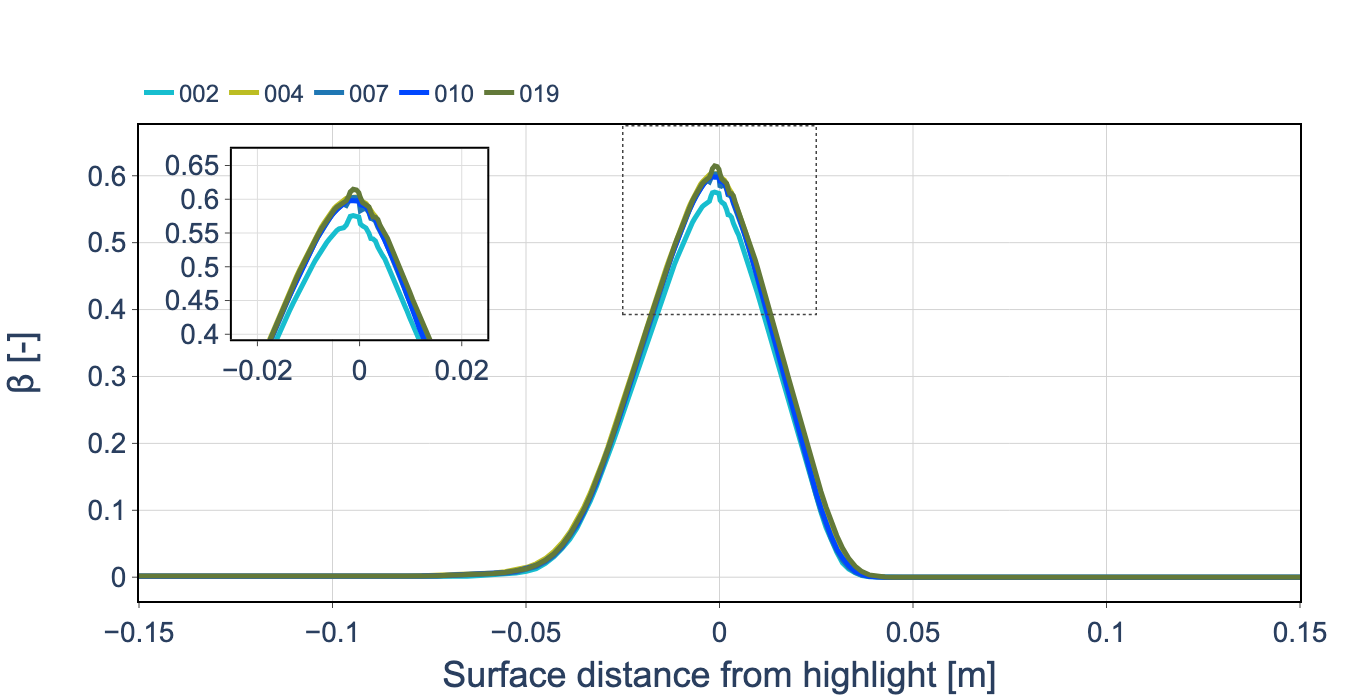
\includegraphics[width=0.96\textwidth]{FIGURES/IMPINGEMENT/tc_oneram6_L1_beta_bins15_vs_s_slice_0p1_roughness_1mm.png}

    \vspace{0.05cm}

    \textbf{$y=0.10$ m}
\end{column}

\begin{column}{0.49\textwidth}
    \centering
    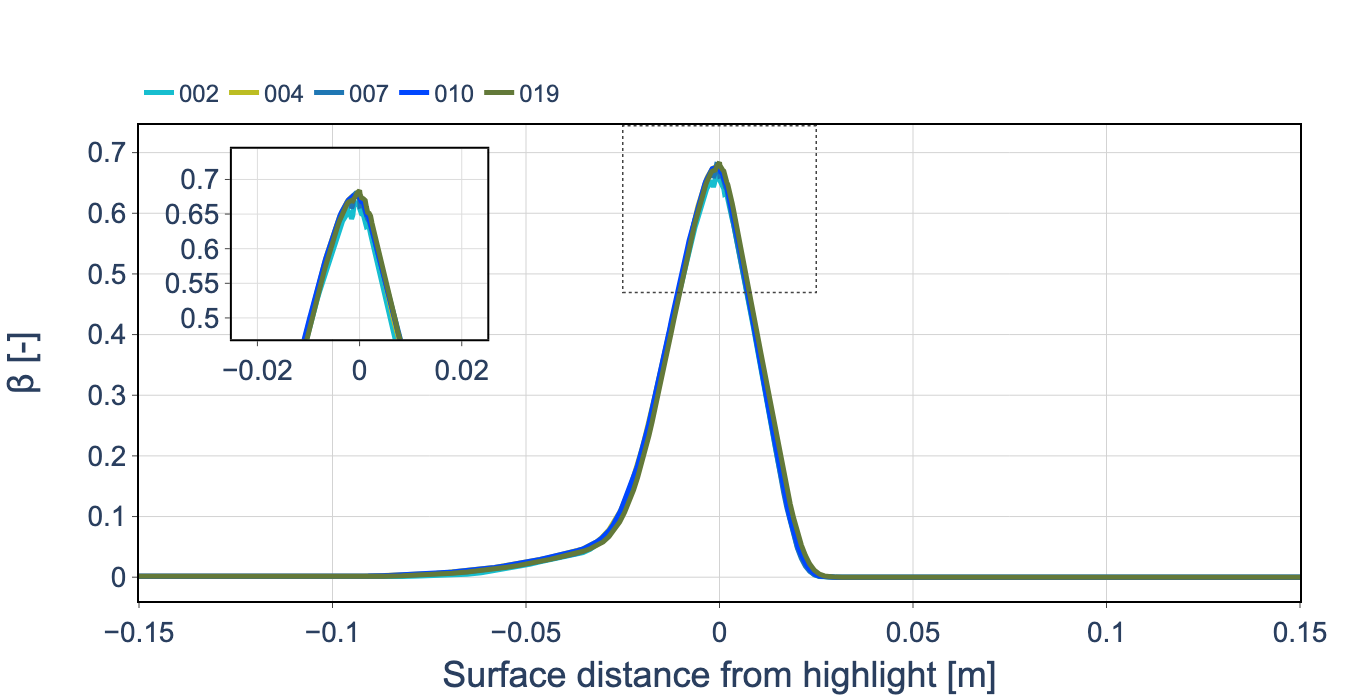
\includegraphics[width=0.96\textwidth]{FIGURES/IMPINGEMENT/tc_oneram6_L1_beta_bins15_vs_s_slice_1p4_roughness_1mm.png}

    \vspace{0.05cm}

    \textbf{$y=1.40$ m}
\end{column}

\end{columns}
}

\vspace{0.10cm}

\begin{block}{\scriptsize Assessment}
\begin{itemize}
    \item Good code-to-code agreement is observed in the collection-efficiency distribution at the representative middle spanwise station ($y=0.75$ m).
    \item The peak magnitude and location are closely clustered across submissions.
    \item<2-> Similar agreement is observed at the inboard and outboard stations.
    \item<2-> Small oscillations near the peak are likely associated with the surface discretization in the highly curved leading-edge region.
\end{itemize}
\end{block}

\end{frame}


% ============================================================
% ONERA M6 -- Water Mass Grid Convergence
% ============================================================

\begin{frame}{\small ONERA M6 -- Water Mass Grid Convergence (15 Bins)}
\scriptsize

{\centering
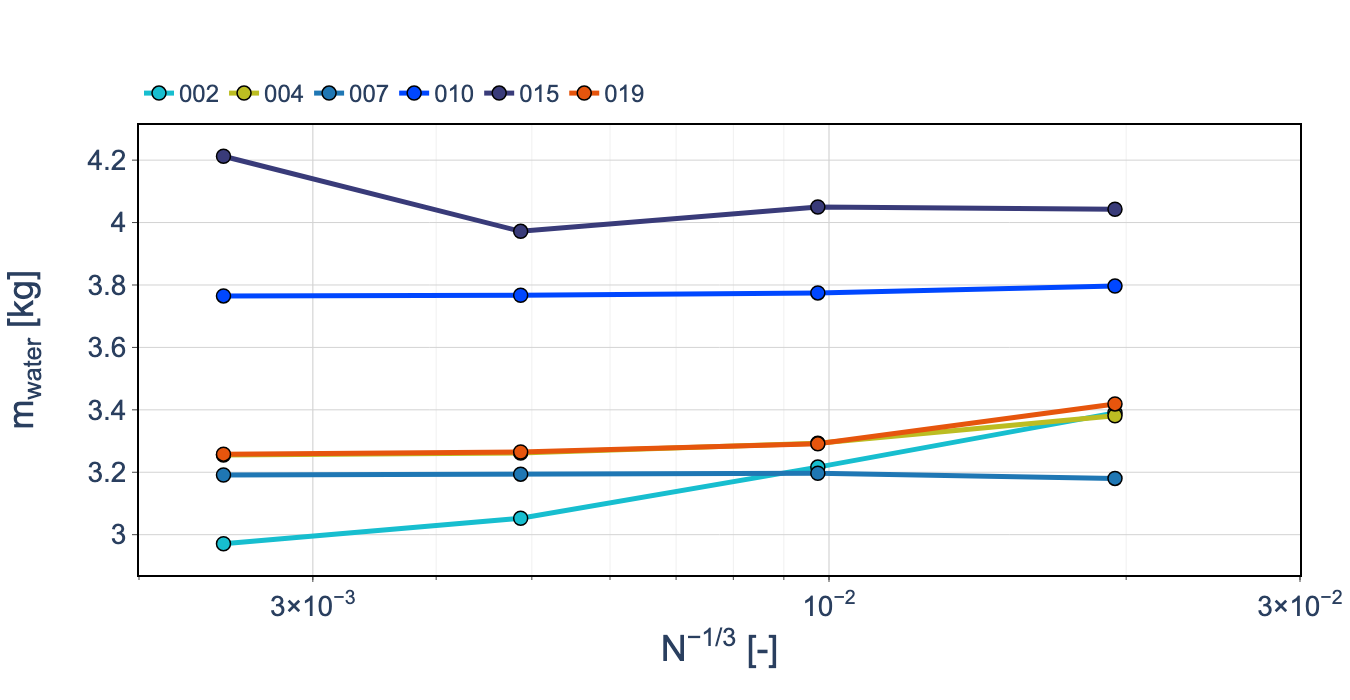
\includegraphics[width=0.48\textwidth]{FIGURES/IMPINGEMENT/tc_oneram6_water_mass_vs_n_1mm_bins15_all_grid_levels.png}
\hfill
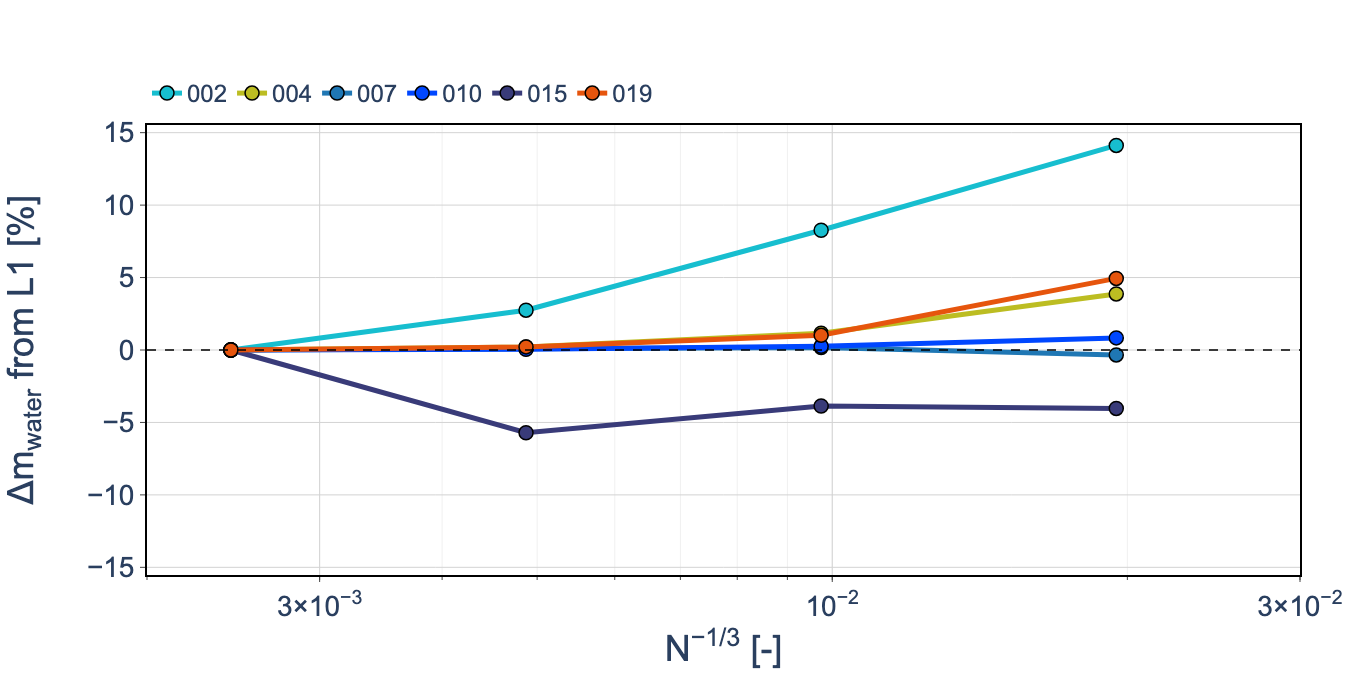
\includegraphics[width=0.48\textwidth]{FIGURES/IMPINGEMENT/tc_oneram6_water_mass_vs_n_1mm_bins15_all_grid_levels_relative_to_l1.png}
\par}

\vspace{0.15cm}

\begin{block}{\scriptsize Assessment}
\begin{itemize}
    \item For the 15-bin distribution, the L1 median water mass is $3.257~\mathrm{kg}$, with an IQR of $0.431~\mathrm{kg}$ ($13.2\%$).
    \item Most submissions exhibit limited sensitivity to spatial grid refinement, with changes generally remaining within approximately $5\%$ of their corresponding L1 predictions.
\end{itemize}
\end{block}

\end{frame}

% ============================================================
% ONERA M6 -- Droplet Distribution Sensitivity
% ============================================================

\begin{frame}{\small ONERA M6 -- Droplet Distribution Sensitivity (L1)}
\scriptsize

\begin{columns}[T,onlytextwidth]

\begin{column}{0.50\textwidth}
    \centering
    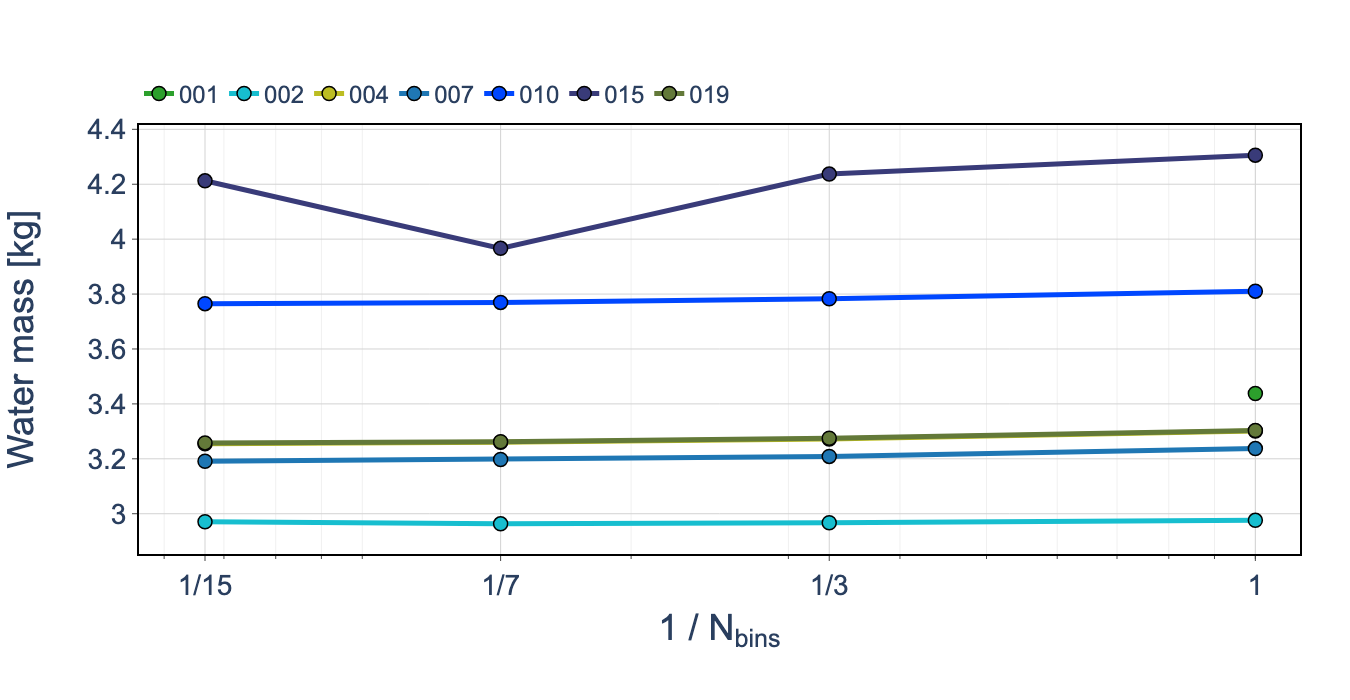
\includegraphics[width=0.96\textwidth]{FIGURES/IMPINGEMENT/tc_oneram6_water_mass_vs_n_1mm_l1_vs_inverse_bins.png}
\end{column}

\begin{column}{0.50\textwidth}
    \centering
    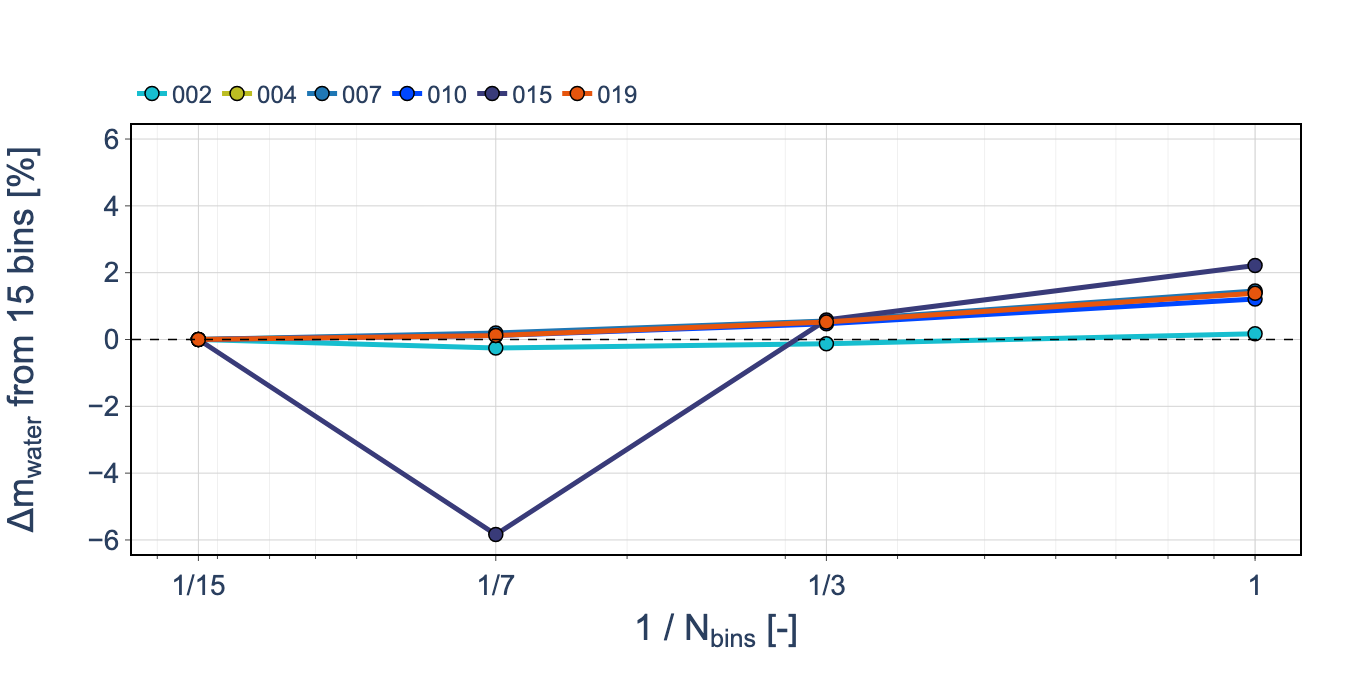
\includegraphics[width=0.96\textwidth]{FIGURES/IMPINGEMENT/tc_oneram6_water_mass_vs_n_1mm_l1_vs_inverse_bins_relative_to_bins15.png}
\end{column}

\end{columns}

\vspace{0.10cm}

\begin{block}{\scriptsize Assessment}
\begin{itemize}
    \item All the distributions produce very similar impinged water masses for most submissions.
    \item Relative differences remain within approximately $2\%$ for most submissions and distributions, with one isolated 7-bin deviation of approximately $6\%$.
    \item The narrow droplet-size range ($6.16$--$33.84~\mu$m around an MVD of $20~\mu$m) contributes to the weak distribution sensitivity.
\end{itemize}
\end{block}

\end{frame}

% ============================================================
% ONERA M6 -- Water-Mass Variability by Droplet Diameter
% ============================================================

\begin{frame}{\small ONERA M6 -- Water-Mass Variability by Droplet Diameter}
\scriptsize

\begin{columns}[c,onlytextwidth]

\begin{column}{0.50\textwidth}
    \centering
    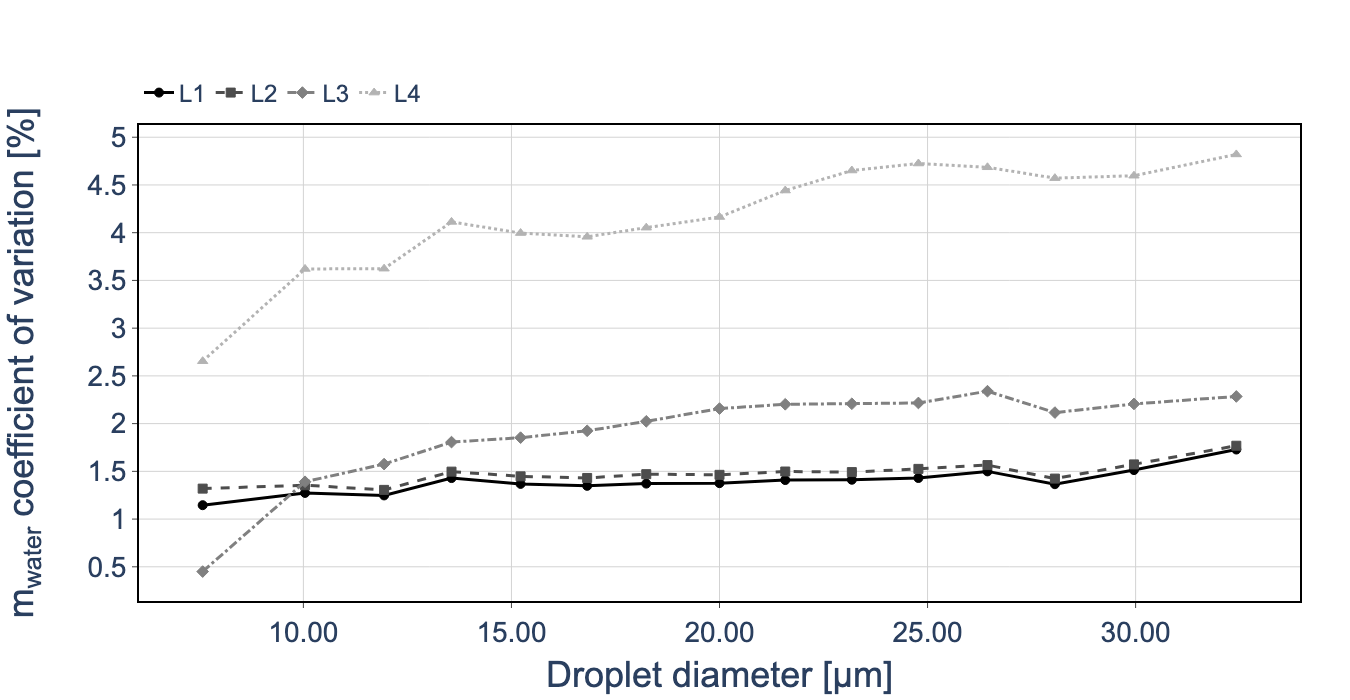
\includegraphics[width=\textwidth]{FIGURES/IMPINGEMENT/tc_oneram6_water_mass_coefficient_of_variation_vs_droplet_diameter_bins15_all_grid_levels.png}
\end{column}

\begin{column}{0.50\textwidth}
    \centering
    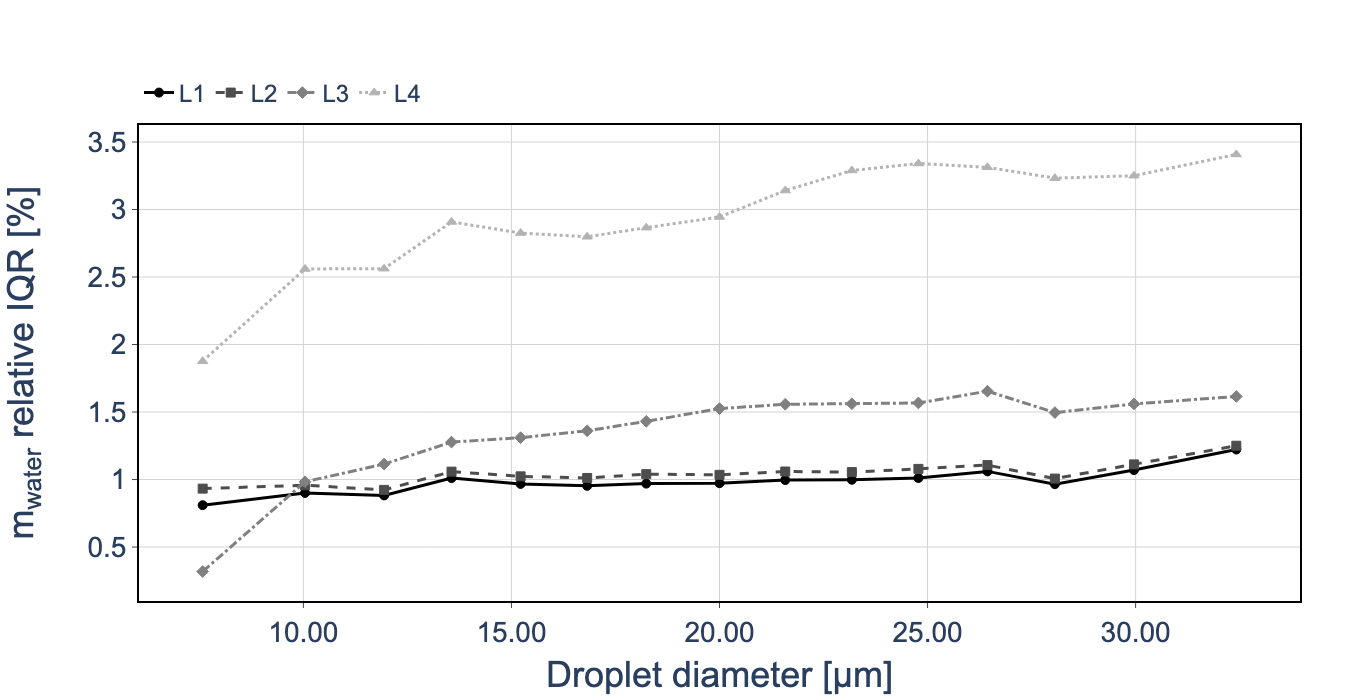
\includegraphics[width=\textwidth]{FIGURES/IMPINGEMENT/tc_oneram6_water_mass_relative_iqr_vs_droplet_diameter_bins15_all_grid_levels.png}
\end{column}

\end{columns}

\vspace{0.15cm}

\begin{block}{\scriptsize Assessment}
\begin{itemize}
    \item On the fine L1 and L2 grids, the code-to-code variability remains low across the entire droplet-diameter range, with relative IQR values generally around $1\%$.
    \item Variability increases on the coarser L3 and L4 grids, indicating a stronger grid-resolution effect than droplet-size dependence.
    \item No pronounced dependence on droplet diameter is observed over the relatively narrow $6.16$--$33.84~\mu$m range, centered around an MVD of $20~\mu$m.
    \item This relatively narrow droplet-size distribution also helps explain the weak sensitivity of the integrated impinged water mass to the number of bins.
\end{itemize}
\end{block}

\end{frame}

% ============================================================
% ONERA M6 -- Impingement Width Grid Convergence
% ============================================================

\begin{frame}{\small ONERA M6 -- Impingement Width Grid Convergence (15 Bins)}
\scriptsize

\begin{columns}[c,onlytextwidth]

\begin{column}{0.49\textwidth}
    \centering
    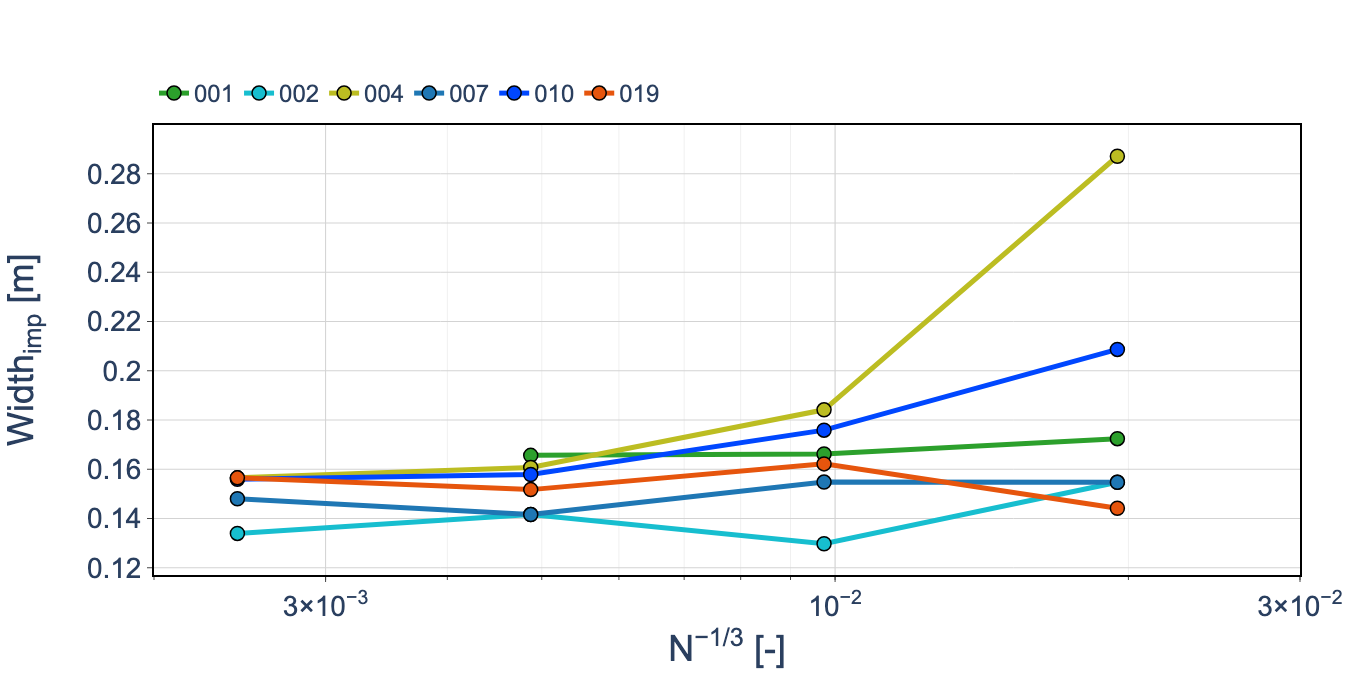
\includegraphics[width=\textwidth]{FIGURES/IMPINGEMENT/tc_oneram6_width_bins15_0_75.png}

    \vspace{-0.10cm}
    \textbf{$y=0.75$ m}
\end{column}

\begin{column}{0.49\textwidth}
    \centering
    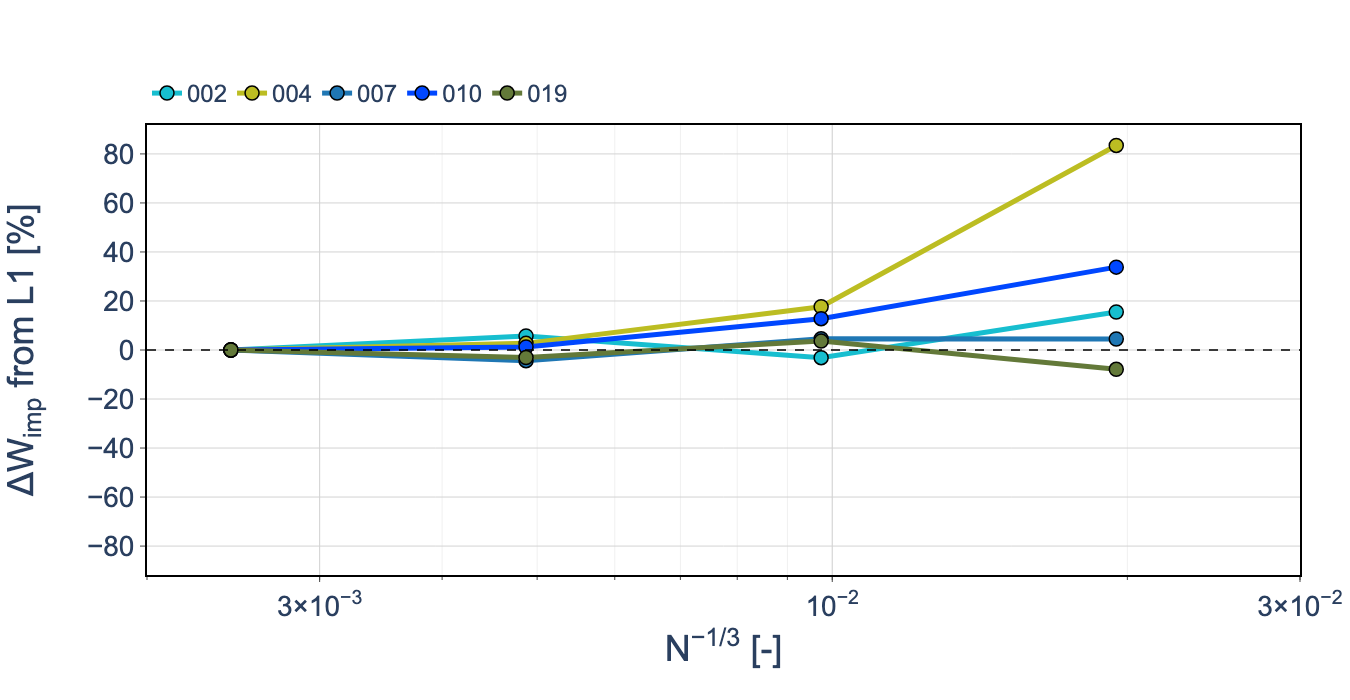
\includegraphics[width=\textwidth]{FIGURES/IMPINGEMENT/tc_oneram6_width_bins15_0_75_relative_to_l1.png}
\end{column}

\end{columns}

\vspace{0.15cm}

\begin{block}{\scriptsize Assessment}
\begin{itemize}
    \item Due to the oscillations observed near the $\beta$ peak, the peak magnitude and position are excluded from the grid-convergence assessment; the impingement width is retained as the primary profile-based metric.
    \item The impingement width is defined from the lower and upper $\beta=0.001$ threshold crossings.
    \item Most submissions show comparatively limited grid sensitivity between L1 and L2.
    \item Larger and non-monotonic deviations are observed on the coarser grids for several submissions, indicating greater sensitivity of the predicted impingement limits to spatial resolution.
\end{itemize}
\end{block}

\end{frame}

% ============================================================
% ONERA M6 -- Impingement Width Distribution Sensitivity
% ============================================================

\begin{frame}{\small ONERA M6 -- Impingement Width Distribution Sensitivity (L1)}
\scriptsize

\begin{columns}[c,onlytextwidth]

\begin{column}{0.49\textwidth}
    \centering
    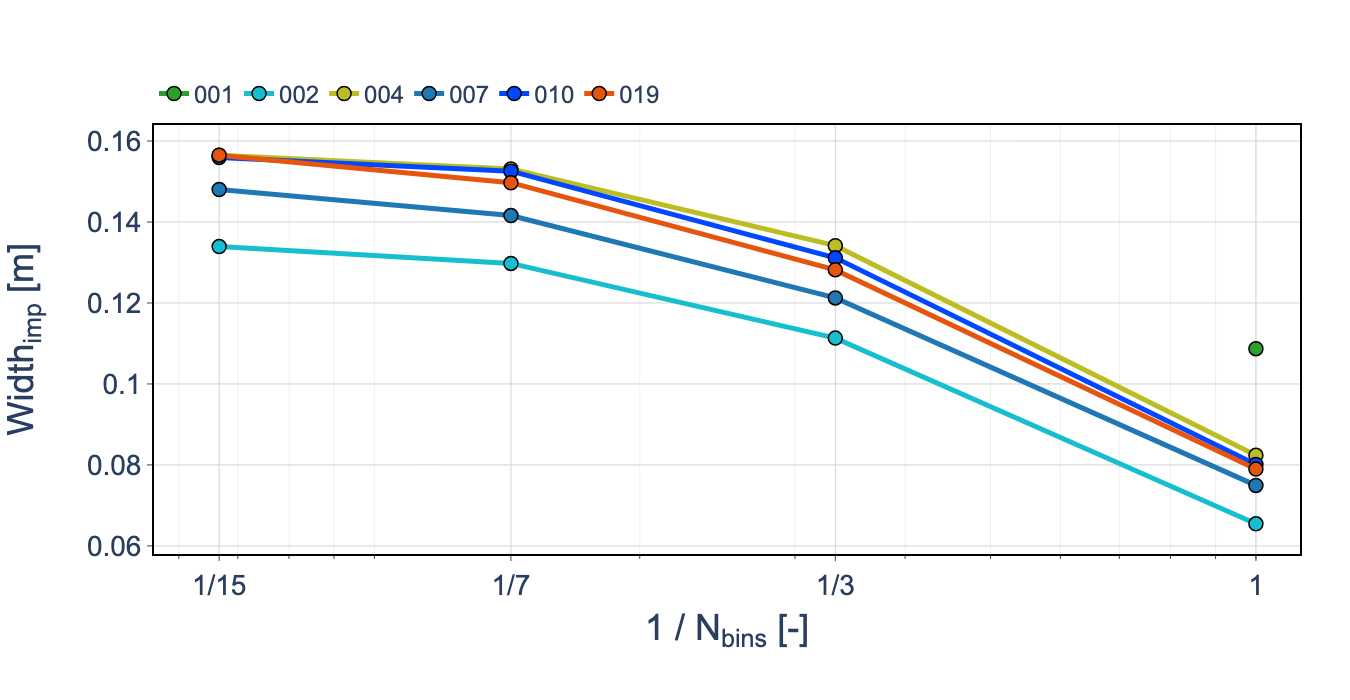
\includegraphics[width=\textwidth]{FIGURES/IMPINGEMENT/tc_oneram6_width_distribution_convergence_l1_0_75.png}

    \vspace{-0.10cm}
    \textbf{$y=0.75$ m}
\end{column}

\begin{column}{0.49\textwidth}
    \centering
    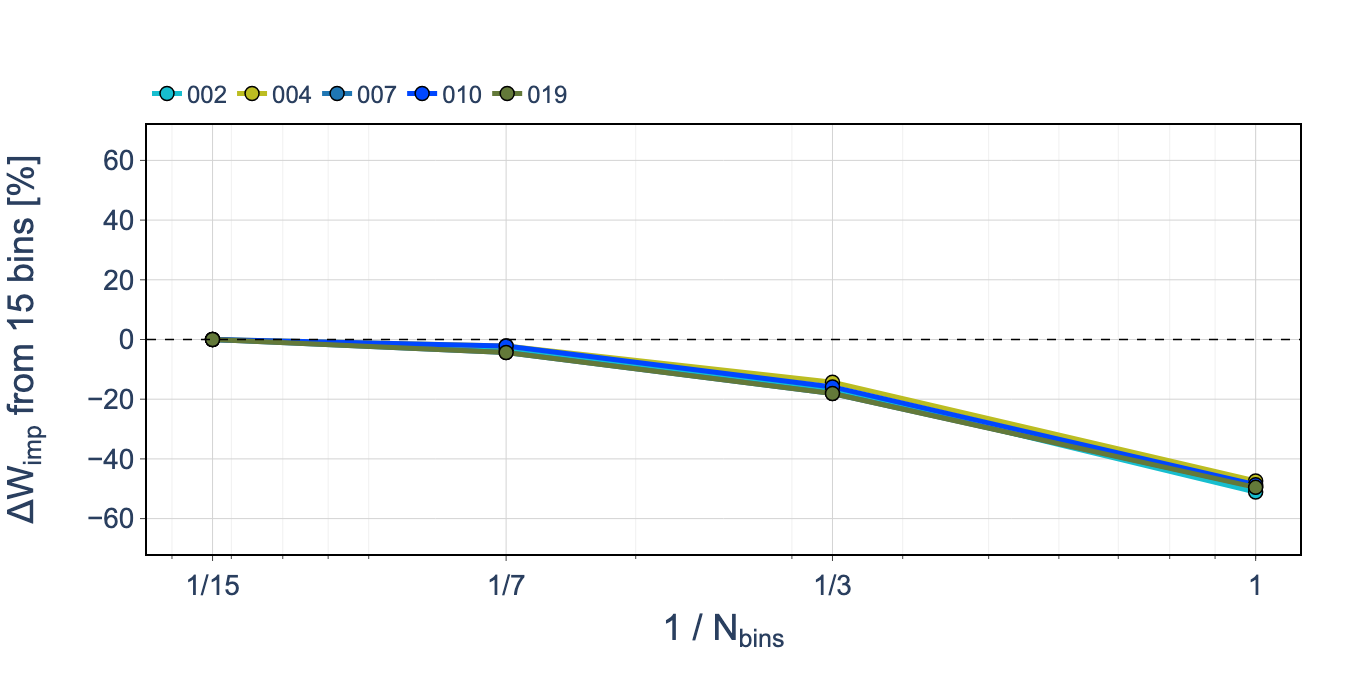
\includegraphics[width=\textwidth]{FIGURES/IMPINGEMENT/tc_oneram6_width_distribution_convergence_l1_0_75_relative_to_bins15.png}
\end{column}

\end{columns}

\vspace{0.15cm}

\begin{block}{\scriptsize Assessment}
\begin{itemize}
    \item The predicted impingement width systematically increases as the droplet distribution is refined from 1 to 15 bins.
    \item A noticeable increase remains between the 7- and 15-bin distributions, indicating that convergence with respect to droplet-distribution resolution has not yet been clearly demonstrated.
    \item In contrast, the integrated impinged water mass varies by only approximately $2\%$ between the single- and 15-bin distributions for most submissions.
    \item Droplet-distribution resolution therefore has a substantially stronger influence on the spatial extent of impingement than on the integrated collected water mass.
\end{itemize}
\end{block}

\end{frame}

% ============================================================
% ONERA M6 -- Droplet Impingement Summary
% ============================================================

\begin{frame}{\small ONERA M6 -- Droplet Impingement Summary}
\scriptsize

\begin{block}{\scriptsize Spatial Grid Convergence}
\begin{itemize}
    \item Collection-efficiency distributions show good code-to-code agreement across the three spanwise stations.
    \item Integrated water mass exhibits limited grid sensitivity for most submissions, while code-to-code differences remain larger.
    \item Impingement limits are more sensitive to spatial resolution, particularly on the coarser grids.
\end{itemize}
\end{block}

\vspace{0.15cm}

\begin{block}{\scriptsize Droplet-Size Distribution}
\begin{itemize}
    \item Integrated water mass is weakly sensitive to droplet discretization; even the single-MVD approximation remains within approximately $2\%$ of the 15-bin prediction for most submissions.
    \item In contrast, impingement width systematically increases from 1 to 15 bins, with convergence not yet clearly demonstrated at 15 bins.
    \item The relatively narrow $6.16$--$33.84~\mu$m range around the $20~\mu$m MVD contributes to the weak sensitivity of the integrated water mass.
\end{itemize}
\end{block}

\vspace{0.15cm}

\begin{alertblock}{\scriptsize Impingement Takeaway}
Integrated water mass can appear converged while the spatial impingement extent remains sensitive to both spatial and droplet-distribution resolution.
\end{alertblock}

\end{frame}
